 
% -- aginst Rich et al. BDSD survey ugriz podaci
% -- Bailer-Jones i S82
% -- Trilegal simulacije s SDSS SED modelima (validacija)
% -- kuglasti skupovi




\section{Implementation: Photo-D pipeline and Tests}

First describe pipeline and implementation choices, then its performance  


% Our method is basically brute-force fitting with some intelligent tricks leveraged to obtain faster execution that will be required for 10B LSST stars. 


\subsection{Accelerated Exhaustive Grid Search Method}
optimized grid search, MCMC, refer to NN paper, also in Discussion

Our fitting procedure is also executed on an adaptive grid, a coarse search over the parameter space is performed first in order to establish the layout of the manifold. However, care is taken that any possible local minima are not missed by appropriately adjusting the step size \magcom{how?}. The located maxima are then explored with a smaller step size (\magcom{adjusted how?}).


\subsection{Markov Chain Monte Carlo Method}

In addition to the approach described here, we also tested Markov Chain Monte Carlo and neural network approaches that will be/are described in forthcoming/published papers.


 XXX Green et al. (2014) used MCMC 


\subsection{Neural Network Method}


\subsection{LSDB and Healpix Implementation} 

% 2) statistics:

The priors are established by partitioning the TRILEGAL galaxy model
\citep{dal_tio_simulating_2022} in healpixels,
and each of the pixel in one-magnitude wide bins in apparent
magnitude.


\subsection{Performance Testing} 

Motivate three parts: simulated photometry, SDSS-Gaia sample and DECam bulge sample. 


\subsubsection{Simulated Data Set}

\begin{figure*}[ht!]
\hskip -0.3in
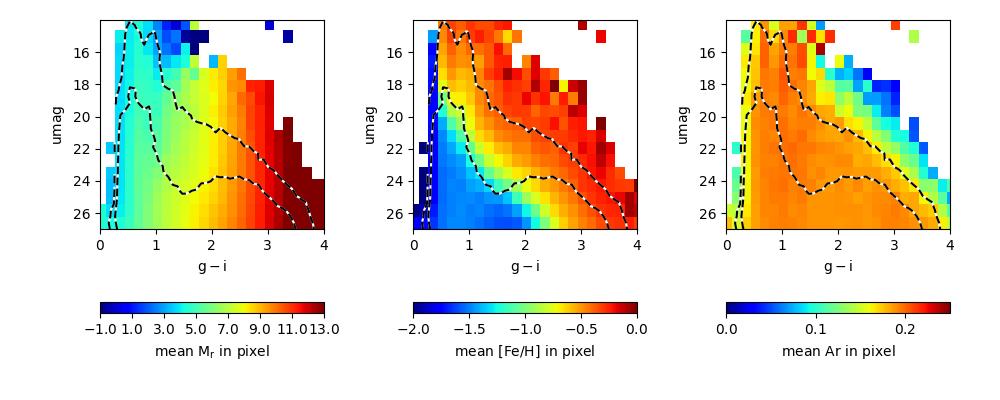
\includegraphics[width=1.08\textwidth,angle=0]{figures/qpBmeans_SDSSpatchRA340-350-simLSST_FeH.png}
\vskip -0.3in
\caption{The mean per-pixel values of absolute magnitude $M_r$,
  metallicity $[Fe/H]$, and interstellar dust extinction along the line of sight in
  the $r$ band, $A_r$, for a TRILEGAL-simulated sample of 283,000 main
  sequence and red giants stars with $r<26$, $340^{\degree} < {\rm R.A.} < 350^{\degree}$
  and $-1.3^{\degree} < \delta < 1.3^{\degree}$
  (a small patch from the SDSS Stripe 82 region). The mean values are
  color-coded according to legends below each panel. Contours
  visualize the sample distribution in each diagram. The strong variation
  of $M_r$ with the $g-i$ color is seen in the left panel. The
  diagonal iso-metallicity boundaries in the middle panel closely correspond to distance
  (in the range from about 1 kpc to about 100 kpc). The values of
  dust extinction, shown in the right panel, are not large because the
  selected field is at high Galactic latitudes (centered on $b = -52^{\degree}$).}
\label{fig:qpBmeans}
\end{figure*}


\begin{figure*}[ht!]
\plotone{qpB_SDSSpatchRA340-350-simLSST_Mr.png}
\plotone{qpB_SDSSpatchRA340-350-simLSST_FeH.png}
\plotone{qpB_SDSSpatchRA340-350-simLSST_Ar.png}
\caption{Performance analysis for estimates of model parameters $M_r$
  (top row),  $[Fe/H]$ (middle row), and $A_r$ (bottom row) in the
  space of $M_r$ and $[Fe/H]$, for the same simulated sample as shown
  in Figure~\ref{fig:qpBmeans}. 
  The left column shows the mean difference per pixel between the true
  and estimated values, the middle column shows scatter per pixel and
  the right column shows the scatter normalized by estimated
  uncertainties. Contours visualize the sample distribution in each
  diagram. Note that for main sequence stars $M_r>4$ and for most
  stars $4 < M_r < 10$. 
\label{fig:perfVStrueParams}}
\end{figure*}


\begin{figure*}[ht!]
\plotone{qpB_estQ_SDSSpatchRA340-350-simLSST_Mr.png}
\plotone{qpB_estQ_SDSSpatchRA340-350-simLSST_FeH.png}
\plotone{qpB_estQ_SDSSpatchRA340-350-simLSST_Ar.png}
\caption{Analogous to Figure~\ref{fig:perfVStrueParams}, except that
  the results are binned in the space of estimated $M_r$ and $[Fe/H]$ parameters.
\label{fig:perfVSestParams}}
\end{figure*}
 



\begin{figure*}[ht!]
\plotone{qpBcmd_SDSSpatchRA340-350-simLSST_Mr.png}
\plotone{qpBcmd_SDSSpatchRA340-350-simLSST_FeH.png}
\plotone{qpBcmd_SDSSpatchRA340-350-simLSST_Ar.png}
\caption{Analogous to Figures~\ref{fig:perfVStrueParams} and \ref{fig:perfVSestParams}
except that the results are binned in the space of 
  of observables: $u$ band magnitude and the $g-i$ color
\label{fig:perfVScmd}}
\end{figure*}





Basic tests of numerics, intrinsic model degeneracies and performance
as a function of photometric signal-to-noise ratio... 

Simulated photometry using color sequences for 10 Gyr isochrone shown in Figure~\ref{fig:augmLocus}. 
and photometric errors expected for LSST coadded depths (Bianco et al. )

Main summary in Table 1 (need proper latex), more details in figures below. 

No trend with u mag, only increase in scatter towards the faint end. 

The distribution of model parameters (absolute magnitude $M_r$,
metallicity $[Fe/H]$, and interstellar dust extinction along the line
of sight in the $r$ band, $A_r$) for the simulated sample in the space
of observables: $u$ band magnitude and the $g-i$ color, is shown in
Figure~\ref{fig:perfVScmd}.

Performance for estimates of model parameters $M_r$, $[Fe/H]$ and
$A_r$ is illustrated in the space of model parameters in Figures~\ref{fig:perfVStrueParams}
and \ref{fig:perfVSestParams}, and in the space of observables in
Figure~\ref{fig:perfVScmd}.  

 

\newpage

{\bf Quantitative summary of the performance of Bayesian method on simulated sample:}
Each column shows the median error, robust standard deviation and the subsample size. 
``mag selected'' refers to a subsample selected by $u < 24$. Low and high $[Fe/H]$ subsamples are
separated at $[Fe/H] = -1$. ``Giants'' are selected by $M_r<4$ and blue/red (i.e., bright/faint) main
sequence stars are separated by $M_r=8$.  

\begin{verbatim}
-----------------------------------------------------------------------------------------------
    FULL SAMPLE:           dMr                      dFeH                         Ar
           all: [ '0.010', '0.28', 275863] [ '0.000', '0.25', 275863] ['0.000', '0.04',275863]
  mag selected: [ '0.000', '0.24',  94161] ['-0.010', '0.14',  94161] ['0.000', '0.04', 94161]
-----------------------------------------------------------------------------------------------
     low [FeH]:            dMr                      dFeH                         Ar
           all: ['-0.020', '0.28',  43470] [ '0.010', '0.14',  43470] ['0.000', '0.06', 43470]
        giants: ['-0.430', '0.51',   9165] ['-0.060', '0.15',   9165] ['0.020', '0.07',  9165]
       blue MS: [ '0.030', '0.23',  33609] [ '0.020', '0.13',  33609] ['0.000', '0.05', 33609]
        red MS: [ '0.040', '0.14',    696] ['-0.060', '0.22',    696] ['0.000', '0.05',   696]
    high [FeH]:            dMr                      dFeH                         Ar
           all: [ '0.020', '0.21',  50691] ['-0.020', '0.14',  50691] ['0.000', '0.04', 50691]
        giants: ['-0.570', '0.91',   5721] ['-0.050', '0.20',   5721] ['0.000', '0.06',  5721]
       blue MS: [ '0.040', '0.20',  32841] [ '0.000', '0.13',  32841] ['0.000', '0.04', 32841]
        red MS: [ '0.060', '0.14',  12129] ['-0.070', '0.16',  12129] ['0.000', '0.02', 12129]
-----------------------------------------------------------------------------------------------
\end{verbatim}



% 3) code testing:

% *** data-based comparisons ***
\subsubsection{SDSS-based Comparison to Gaia's Distance Scale} 


\begin{figure*}[ht!]
\plotone{gaiaStripe82plot1.png}
\caption{Analysis of the difference between Gaia's geometric (trigonometric) absolute magnitudes and photometric magnitudes
  derived from SDSS colors. Symbols show a sample of 33,186 stars with the parallax signal-to-noise ratio above 10, absolute
  magnitude MrGeo$>$4 and MrPho$>$4 , and SDSS-based $u<21$ and $0.2 < g-r < 0.6$. The median magnitude difference is
  $-0.01$ mag, with a scatter of 0.28 mag. The four panel illustrate variation of the binned median (red circles) and scatter (red
  lines) with the $u$-band magnitude, the parallax signal-to-noise ratio, SDSS $g-r$ color, and photometric metallicity.} 
\label{fig:gaiasdss1}
\end{figure*}


\begin{figure*}[ht!]
\plotone{gaiaStripe82plot2.png}
\caption{Analysis of the difference between Gaia's photometric (color-based) absolute magnitudes and photometric magnitudes
  derived from SDSS colors. Symbols show a sample of 165,834 stars with absolute magnitude MrPho$>$4, and SDSS-based $u<21$
  and $0.2 < g-r < 0.6$. The median magnitude difference is $-0.05$ mag, with a scatter of 0.32 mag. The four panel illustrate
  variation of the binned median (red circles) and scatter (red lines) with the $u$-band magnitude, SDSS $u-g$ and $g-r$ colors,
  and photometric metallicity.}
\label{fig:gaiasdss2}
\end{figure*}



Stripe 82 vs. Gaia...  It works great for $0.2 < g-r < 0.6$ stars using directly photometric $[Fe/H]$ and $M_r$ expressions from the
Tomography papers. See Figures~\ref{fig:gaiasdss1} and \ref{fig:gaiasdss2}. Does it work within the Bayesian framework? Does it work outside this color range? 




\subsubsection{Performance in Bulge Fields} 

Bulge BDSD sample...  Different photometric system, differences compared to model colors. Should we descope it? 

